% Created by tikzDevice version 0.10.1 on 2016-07-26 22:19:47
% !TEX encoding = UTF-8 Unicode
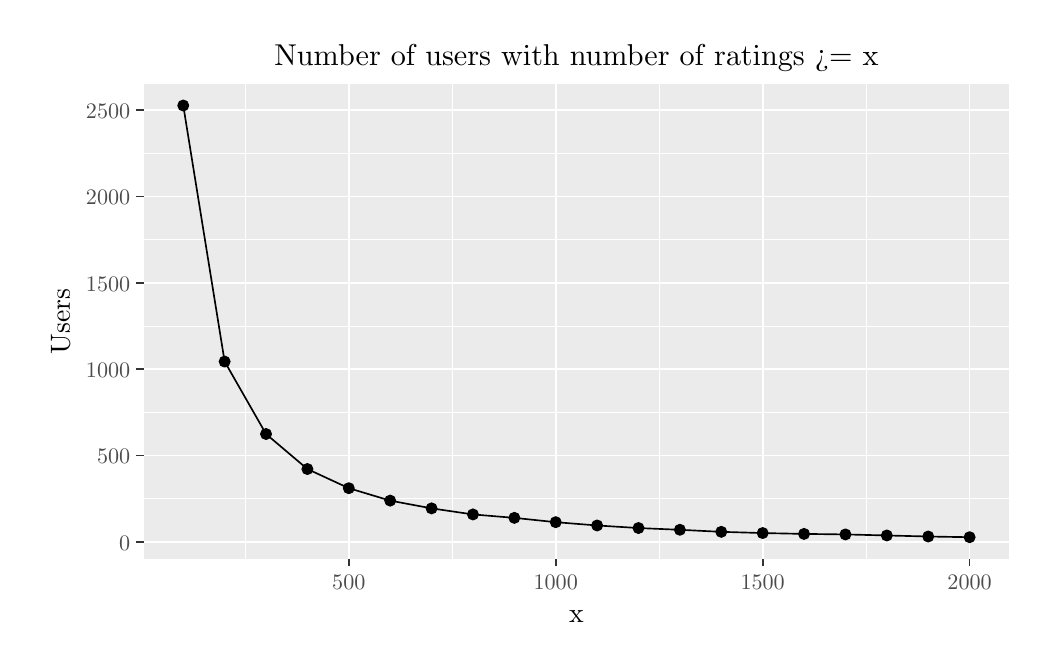
\begin{tikzpicture}[x=1pt,y=1pt]
\definecolor{fillColor}{RGB}{255,255,255}
\path[use as bounding box,fill=fillColor,fill opacity=0.00] (0,0) rectangle (360.07,222.54);
\begin{scope}
\path[clip] (  0.00,  0.00) rectangle (360.07,222.54);
\definecolor{drawColor}{RGB}{255,255,255}
\definecolor{fillColor}{RGB}{255,255,255}

\path[draw=drawColor,line width= 0.6pt,line join=round,line cap=round,fill=fillColor] (  0.00,  0.00) rectangle (360.07,222.54);
\end{scope}
\begin{scope}
\path[clip] ( 42.01, 30.62) rectangle (354.57,202.21);
\definecolor{fillColor}{gray}{0.92}

\path[fill=fillColor] ( 42.01, 30.62) rectangle (354.57,202.21);
\definecolor{drawColor}{RGB}{255,255,255}

\path[draw=drawColor,line width= 0.3pt,line join=round] ( 42.01, 52.39) --
	(354.57, 52.39);

\path[draw=drawColor,line width= 0.3pt,line join=round] ( 42.01, 83.56) --
	(354.57, 83.56);

\path[draw=drawColor,line width= 0.3pt,line join=round] ( 42.01,114.74) --
	(354.57,114.74);

\path[draw=drawColor,line width= 0.3pt,line join=round] ( 42.01,145.91) --
	(354.57,145.91);

\path[draw=drawColor,line width= 0.3pt,line join=round] ( 42.01,177.08) --
	(354.57,177.08);

\path[draw=drawColor,line width= 0.3pt,line join=round] ( 78.65, 30.62) --
	( 78.65,202.21);

\path[draw=drawColor,line width= 0.3pt,line join=round] (153.43, 30.62) --
	(153.43,202.21);

\path[draw=drawColor,line width= 0.3pt,line join=round] (228.20, 30.62) --
	(228.20,202.21);

\path[draw=drawColor,line width= 0.3pt,line join=round] (302.98, 30.62) --
	(302.98,202.21);

\path[draw=drawColor,line width= 0.6pt,line join=round] ( 42.01, 36.80) --
	(354.57, 36.80);

\path[draw=drawColor,line width= 0.6pt,line join=round] ( 42.01, 67.98) --
	(354.57, 67.98);

\path[draw=drawColor,line width= 0.6pt,line join=round] ( 42.01, 99.15) --
	(354.57, 99.15);

\path[draw=drawColor,line width= 0.6pt,line join=round] ( 42.01,130.32) --
	(354.57,130.32);

\path[draw=drawColor,line width= 0.6pt,line join=round] ( 42.01,161.49) --
	(354.57,161.49);

\path[draw=drawColor,line width= 0.6pt,line join=round] ( 42.01,192.67) --
	(354.57,192.67);

\path[draw=drawColor,line width= 0.6pt,line join=round] (116.04, 30.62) --
	(116.04,202.21);

\path[draw=drawColor,line width= 0.6pt,line join=round] (190.81, 30.62) --
	(190.81,202.21);

\path[draw=drawColor,line width= 0.6pt,line join=round] (265.59, 30.62) --
	(265.59,202.21);

\path[draw=drawColor,line width= 0.6pt,line join=round] (340.36, 30.62) --
	(340.36,202.21);
\definecolor{drawColor}{RGB}{0,0,0}

\path[draw=drawColor,line width= 0.6pt,line join=round] ( 56.22,194.41) --
	( 71.17,101.89) --
	( 86.13, 75.71) --
	(101.08, 63.05) --
	(116.04, 56.13) --
	(130.99, 51.64) --
	(145.95, 48.84) --
	(160.90, 46.65) --
	(175.86, 45.41) --
	(190.81, 43.85) --
	(205.77, 42.66) --
	(220.72, 41.73) --
	(235.68, 41.10) --
	(250.63, 40.36) --
	(265.59, 39.92) --
	(280.54, 39.61) --
	(295.50, 39.42) --
	(310.45, 39.05) --
	(325.41, 38.67) --
	(340.36, 38.42);
\definecolor{fillColor}{RGB}{0,0,0}

\path[draw=drawColor,line width= 0.4pt,line join=round,line cap=round,fill=fillColor] ( 56.22,194.41) circle (  1.96);

\path[draw=drawColor,line width= 0.4pt,line join=round,line cap=round,fill=fillColor] ( 71.17,101.89) circle (  1.96);

\path[draw=drawColor,line width= 0.4pt,line join=round,line cap=round,fill=fillColor] ( 86.13, 75.71) circle (  1.96);

\path[draw=drawColor,line width= 0.4pt,line join=round,line cap=round,fill=fillColor] (101.08, 63.05) circle (  1.96);

\path[draw=drawColor,line width= 0.4pt,line join=round,line cap=round,fill=fillColor] (116.04, 56.13) circle (  1.96);

\path[draw=drawColor,line width= 0.4pt,line join=round,line cap=round,fill=fillColor] (130.99, 51.64) circle (  1.96);

\path[draw=drawColor,line width= 0.4pt,line join=round,line cap=round,fill=fillColor] (145.95, 48.84) circle (  1.96);

\path[draw=drawColor,line width= 0.4pt,line join=round,line cap=round,fill=fillColor] (160.90, 46.65) circle (  1.96);

\path[draw=drawColor,line width= 0.4pt,line join=round,line cap=round,fill=fillColor] (175.86, 45.41) circle (  1.96);

\path[draw=drawColor,line width= 0.4pt,line join=round,line cap=round,fill=fillColor] (190.81, 43.85) circle (  1.96);

\path[draw=drawColor,line width= 0.4pt,line join=round,line cap=round,fill=fillColor] (205.77, 42.66) circle (  1.96);

\path[draw=drawColor,line width= 0.4pt,line join=round,line cap=round,fill=fillColor] (220.72, 41.73) circle (  1.96);

\path[draw=drawColor,line width= 0.4pt,line join=round,line cap=round,fill=fillColor] (235.68, 41.10) circle (  1.96);

\path[draw=drawColor,line width= 0.4pt,line join=round,line cap=round,fill=fillColor] (250.63, 40.36) circle (  1.96);

\path[draw=drawColor,line width= 0.4pt,line join=round,line cap=round,fill=fillColor] (265.59, 39.92) circle (  1.96);

\path[draw=drawColor,line width= 0.4pt,line join=round,line cap=round,fill=fillColor] (280.54, 39.61) circle (  1.96);

\path[draw=drawColor,line width= 0.4pt,line join=round,line cap=round,fill=fillColor] (295.50, 39.42) circle (  1.96);

\path[draw=drawColor,line width= 0.4pt,line join=round,line cap=round,fill=fillColor] (310.45, 39.05) circle (  1.96);

\path[draw=drawColor,line width= 0.4pt,line join=round,line cap=round,fill=fillColor] (325.41, 38.67) circle (  1.96);

\path[draw=drawColor,line width= 0.4pt,line join=round,line cap=round,fill=fillColor] (340.36, 38.42) circle (  1.96);
\end{scope}
\begin{scope}
\path[clip] (  0.00,  0.00) rectangle (360.07,222.54);
\definecolor{drawColor}{gray}{0.30}

\node[text=drawColor,anchor=base east,inner sep=0pt, outer sep=0pt, scale=  0.80] at ( 37.06, 33.79) {0};

\node[text=drawColor,anchor=base east,inner sep=0pt, outer sep=0pt, scale=  0.80] at ( 37.06, 64.96) {500};

\node[text=drawColor,anchor=base east,inner sep=0pt, outer sep=0pt, scale=  0.80] at ( 37.06, 96.13) {1000};

\node[text=drawColor,anchor=base east,inner sep=0pt, outer sep=0pt, scale=  0.80] at ( 37.06,127.31) {1500};

\node[text=drawColor,anchor=base east,inner sep=0pt, outer sep=0pt, scale=  0.80] at ( 37.06,158.48) {2000};

\node[text=drawColor,anchor=base east,inner sep=0pt, outer sep=0pt, scale=  0.80] at ( 37.06,189.65) {2500};
\end{scope}
\begin{scope}
\path[clip] (  0.00,  0.00) rectangle (360.07,222.54);
\definecolor{drawColor}{gray}{0.20}

\path[draw=drawColor,line width= 0.6pt,line join=round] ( 39.26, 36.80) --
	( 42.01, 36.80);

\path[draw=drawColor,line width= 0.6pt,line join=round] ( 39.26, 67.98) --
	( 42.01, 67.98);

\path[draw=drawColor,line width= 0.6pt,line join=round] ( 39.26, 99.15) --
	( 42.01, 99.15);

\path[draw=drawColor,line width= 0.6pt,line join=round] ( 39.26,130.32) --
	( 42.01,130.32);

\path[draw=drawColor,line width= 0.6pt,line join=round] ( 39.26,161.49) --
	( 42.01,161.49);

\path[draw=drawColor,line width= 0.6pt,line join=round] ( 39.26,192.67) --
	( 42.01,192.67);
\end{scope}
\begin{scope}
\path[clip] (  0.00,  0.00) rectangle (360.07,222.54);
\definecolor{drawColor}{gray}{0.20}

\path[draw=drawColor,line width= 0.6pt,line join=round] (116.04, 27.87) --
	(116.04, 30.62);

\path[draw=drawColor,line width= 0.6pt,line join=round] (190.81, 27.87) --
	(190.81, 30.62);

\path[draw=drawColor,line width= 0.6pt,line join=round] (265.59, 27.87) --
	(265.59, 30.62);

\path[draw=drawColor,line width= 0.6pt,line join=round] (340.36, 27.87) --
	(340.36, 30.62);
\end{scope}
\begin{scope}
\path[clip] (  0.00,  0.00) rectangle (360.07,222.54);
\definecolor{drawColor}{gray}{0.30}

\node[text=drawColor,anchor=base,inner sep=0pt, outer sep=0pt, scale=  0.80] at (116.04, 19.64) {500};

\node[text=drawColor,anchor=base,inner sep=0pt, outer sep=0pt, scale=  0.80] at (190.81, 19.64) {1000};

\node[text=drawColor,anchor=base,inner sep=0pt, outer sep=0pt, scale=  0.80] at (265.59, 19.64) {1500};

\node[text=drawColor,anchor=base,inner sep=0pt, outer sep=0pt, scale=  0.80] at (340.36, 19.64) {2000};
\end{scope}
\begin{scope}
\path[clip] (  0.00,  0.00) rectangle (360.07,222.54);
\definecolor{drawColor}{RGB}{0,0,0}

\node[text=drawColor,anchor=base,inner sep=0pt, outer sep=0pt, scale=  1.00] at (198.29,  7.70) {x};
\end{scope}
\begin{scope}
\path[clip] (  0.00,  0.00) rectangle (360.07,222.54);
\definecolor{drawColor}{RGB}{0,0,0}

\node[text=drawColor,rotate= 90.00,anchor=base,inner sep=0pt, outer sep=0pt, scale=  1.00] at ( 15.24,116.42) {Users};
\end{scope}
\begin{scope}
\path[clip] (  0.00,  0.00) rectangle (360.07,222.54);
\definecolor{drawColor}{RGB}{0,0,0}

\node[text=drawColor,anchor=base,inner sep=0pt, outer sep=0pt, scale=  1.09] at (198.29,208.81) {Number of users with number of ratings >= x};
\end{scope}
\end{tikzpicture}
